\documentclass[10pt,border=0pt]{standalone}
% Shared by every standalone figure in this folder. Each figure is built once
% (make figures) and the same PDF is used by the report and, exported as PNG,
% by the README. Times text and 10pt sizes match IEEEtran, so the report
% includes each PDF at its natural size and no font is rescaled. Every
% picture draws its own white background of exactly the width it is placed
% at: 252pt for one column, 516pt for both.
\usepackage{mathptmx}
\usepackage{tikz}
\usetikzlibrary{arrows.meta,positioning,calc,fit,backgrounds}
\usepackage{pgfplots}
\pgfplotsset{compat=1.18}
\usepgfplotslibrary{groupplots}
% Reproducible bytes: no dates or random ids in the PDF.
\pdfinfoomitdate=1
\pdftrailerid{}
\pdfsuppressptexinfo=-1
\newlength{\colw}\setlength{\colw}{252pt}
\newlength{\textw}\setlength{\textw}{516pt}
\tikzset{
  every node/.style={font=\footnotesize},
  line/.style={draw=black!70, line width=0.6pt},
  arr/.style={line, -{Latex[length=4pt,width=3.4pt]}},
  box/.style={draw=black!55, line width=0.5pt, rounded corners=2pt, align=center,
    inner sep=2.5pt, minimum height=22pt},
  exec/.style={box, fill=blue!7},
  stage/.style={box, fill=orange!10},
  eval/.style={box, fill=green!9},
  store/.style={box, fill=black!7, rounded corners=0pt},
  note/.style={font=\scriptsize\itshape, text=black!75, align=center,
    execute at begin node={\hyphenpenalty=10000\exhyphenpenalty=10000}},
  frame/.style={draw=black!45, dashed, line width=0.5pt, rounded corners=3pt},
}
\newcommand{\figbackground}[2]{%
  \fill[white] (0,0) rectangle (#1,-#2);
  \useasboundingbox (0,0) rectangle (#1,-#2);}

% The gate, drawn from the code:
%   per-metric verdict  src/aire/regression/compare.py (_verdict, _apply_statistics:
%                       min_pairs, McNemar for 0/1 metrics, paired bootstrap
%                       otherwise, raw p decides, Holm-adjusted p is reported)
%   exit codes          src/aire/regression/gate.py
%   PR check            .github/workflows/eval-pr.yml, src/aire/ci/pr_check.py
%   PR comment          .github/workflows/eval-pr-comment.yml
\begin{document}
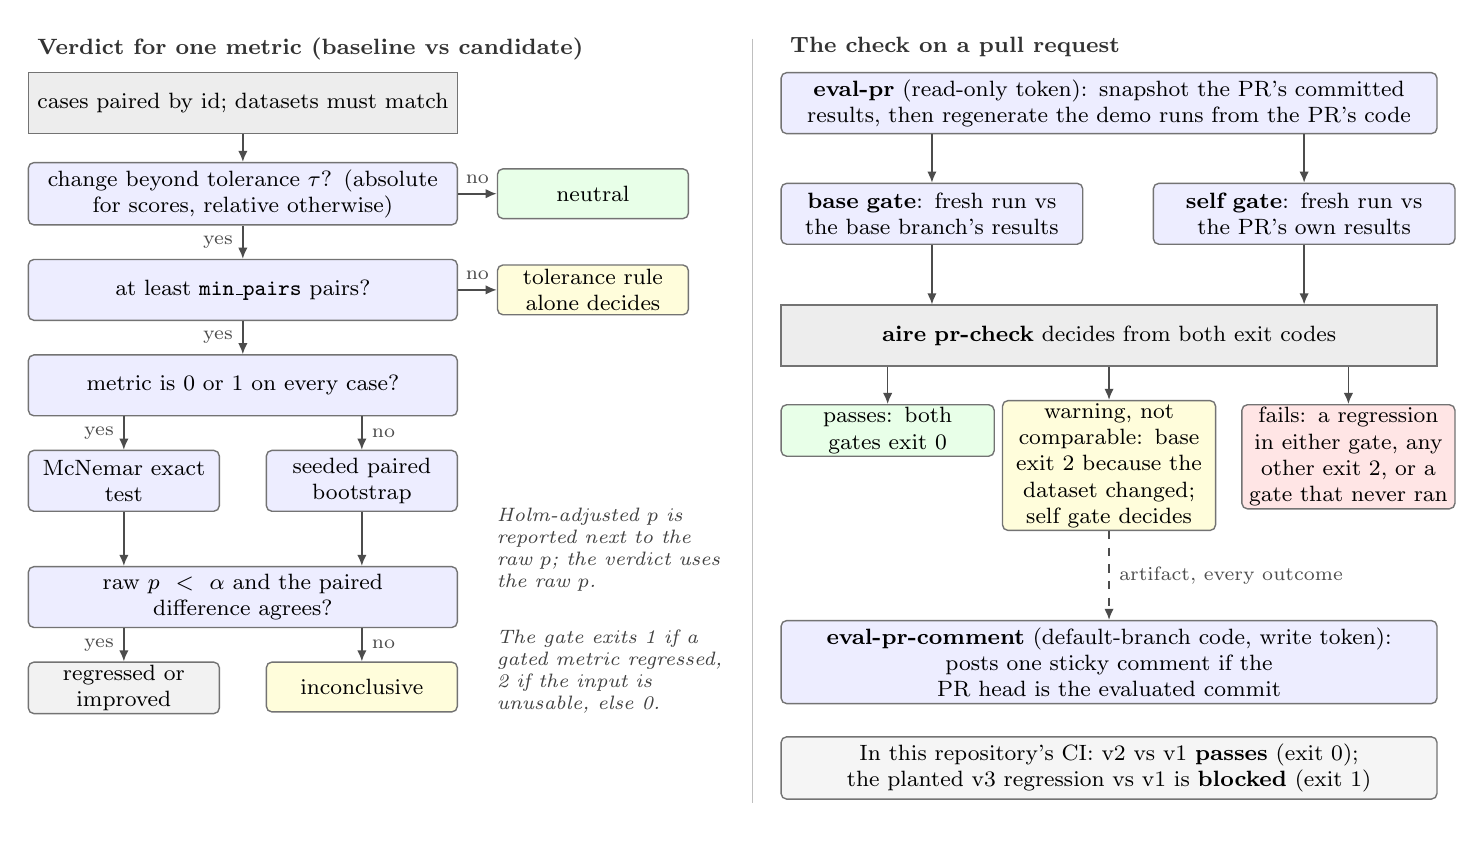
\begin{tikzpicture}[x=1pt,y=1pt]
\figbackground{516}{284}
\tikzset{
  head/.style={font=\footnotesize\bfseries, text=black!80},
  ask/.style={exec, text width=150pt},
  good/.style={eval, text width=64pt, minimum height=18pt, inner ysep=1pt},
  bad/.style={box, fill=red!10, text width=64pt, minimum height=18pt, inner ysep=1pt},
  mid/.style={box, fill=yellow!14, text width=64pt, minimum height=18pt, inner ysep=1pt},
  yes/.style={font=\scriptsize, text=black!70},
}
% Left panel: the verdict for one metric
\node[head, anchor=north west] at (0,0) {Verdict for one metric (baseline vs candidate)};
\node[store, text width=150pt, anchor=north west] (pair) at (0,-16)
  {cases paired by id; datasets must match};
\node[ask, below=10pt of pair] (tol) {change beyond tolerance $\tau$? (absolute\\for scores, relative otherwise)};
\node[good, right=14pt of tol] (neutral) {neutral};
\node[ask, below=12pt of tol] (few) {at least \texttt{min\_pairs} pairs?};
\node[mid, right=14pt of few, text width=64pt] (point) {tolerance rule\\alone decides};
\node[ask, below=12pt of few] (binary) {metric is 0 or 1 on every case?};
\node[exec, text width=64pt, anchor=north west] (mcn) at ($(binary.south west) + (0,-12)$)
  {McNemar exact\\test};
\node[exec, text width=64pt, anchor=north east] (boot) at ($(binary.south east) + (0,-12)$)
  {seeded paired\\bootstrap};
\node[ask, anchor=north west] (sig) at ($(binary.south west) + (0,-54)$)
  {raw $p < \alpha$ and the paired\\difference agrees?};
\node[box, fill=black!5, anchor=north west, text width=64pt, minimum height=18pt, inner ysep=1pt] (moved) at ($(sig.south west) + (0,-12)$)
  {regressed or\\improved};
\node[mid, anchor=north east] (inc) at ($(sig.south east) + (0,-12)$) {inconclusive};
\draw[arr] (pair) -- (tol);
\draw[arr] (tol) -- (neutral) node[midway, above, yes] {no};
\draw[arr] (tol) -- (few) node[midway, left, yes] {yes};
\draw[arr] (few) -- (point) node[midway, above, yes] {no};
\draw[arr] (few) -- (binary) node[midway, left, yes] {yes};
\draw[arr] (binary.south -| mcn) -- (mcn) node[midway, left, yes] {yes};
\draw[arr] (binary.south -| boot) -- (boot) node[midway, right, yes] {no};
\draw[arr] (mcn.south) -- (mcn.south |- sig.north);
\draw[arr] (boot.south) -- (boot.south |- sig.north);
\draw[arr] (sig.south -| moved) -- (moved) node[midway, left, yes] {yes};
\draw[arr] (sig.south -| inc) -- (inc) node[midway, right, yes] {no};
\node[note, text width=86pt, anchor=north west, align=left] at (166,-170)
  {Holm-adjusted $p$ is reported next to the raw $p$; the verdict uses the raw $p$.};
\node[note, text width=86pt, anchor=north west, align=left] at (166,-214)
  {The gate exits 1 if a gated metric regressed, 2 if the input is unusable, else 0.};

% Right panel: the check on a pull request
\draw[black!25] (262,-4) -- (262,-280);
\node[head, anchor=north west] at (272,0) {The check on a pull request};
\node[exec, text width=232pt, anchor=north west] (pr) at (272,-16)
  {\textbf{eval-pr} (read-only token): snapshot the PR's committed\\
   results, then regenerate the demo runs from the PR's code};
\node[exec, text width=104pt, anchor=north west] (base) at (272,-56)
  {\textbf{base gate}: fresh run vs\\the base branch's results};
\node[exec, text width=104pt, anchor=north east] (self) at (516,-56)
  {\textbf{self gate}: fresh run vs\\the PR's own results};
\draw[arr] (pr.south -| base) -- (base);
\draw[arr] (pr.south -| self) -- (self);
\node[store, text width=232pt, anchor=north west] (check) at (272,-100)
  {\textbf{aire pr-check} decides from both exit codes};
\draw[arr] (base) -- (base |- check.north);
\draw[arr] (self) -- (self |- check.north);
\node[good, text width=72pt, anchor=north west] (pass) at (272,-136)
  {passes: both\\gates exit 0};
\node[mid, text width=72pt, anchor=north] (warn) at ($(check.south) + (0,-12)$)
  {warning, not\\comparable: base\\exit 2 because the\\dataset changed;\\self gate decides};
\node[bad, text width=72pt, anchor=north east] (fail) at (516,-136)
  {fails: a regression\\in either gate, any\\other exit 2, or a\\gate that never ran};
\draw[arr] (check.south -| pass) -- (pass);
\draw[arr] (check.south) -- (warn);
\draw[arr] (check.south -| fail) -- (fail);
\node[exec, text width=232pt, anchor=north west] (comment) at (272,-214)
  {\textbf{eval-pr-comment} (default-branch code, write token):\\
   posts one sticky comment if the PR head is the evaluated commit};
\draw[arr, dashed] (warn.south) -- (warn.south |- comment.north)
  node[midway, right, yes] {artifact, every outcome};
\node[box, fill=black!4, text width=232pt, anchor=north west] (demo) at (272,-256)
  {In this repository's CI: v2 vs v1 \textbf{passes} (exit 0);\\
   the planted v3 regression vs v1 is \textbf{blocked} (exit 1)};
\end{tikzpicture}
\end{document}
